\section{Hardware}

This section is dedicated to show all the electronic components we chose and how they work together. As described earlier the PCB containing all the components will be manufactured by Seeedstudio. They manufacture PCBs with other hardware components and they sell quite a number of different breakout boards and other developpement parts. A request made by CHIC managing team was to source as many components as possible at Seeedstudio. Of course not all components we needed were available by them so some of the components are from different sources.

We were basically going to build a tablet. It didn't need to have the power of high end tablets of today but it still was quite a challenge. At first we were thinking it would be possible to take an open source ARM chip devellopment board, devellop our application and then take the schematics and rebuild a whole board including the processor, memory, etc.. plus all our peripherals and build the whole device from scratch. But we quickly understood that it was much too complicated to do in a semester. So we decided to take an existing board and build an add-on board hosting our additionnal components.

There are a number of different devellopment/tinkering boards out there. The most famous one might be the raspberry Pi, although quite capable it seemed a little limited for our application (clocked at 700 mhz for the raspberry pi 1). Another problem was that the raspberry pi is not completely open source. Indeed its schematics and gerber files are not available. At the beginning of the project thinking we might build the whole board up from scratch it was necessary for us to work with a totally open source platform which we could build upon.

So we looked into one of the other famous board: the beagle bone black. Which we will further refer to as the BBB. This board clocked at 1 GHz seemed quite capable. There was lots of documentation, a wide community, and especially it is completelly open source hardware and software. This is what we went for.

In fig.\ref{fig:hardware dependencies} we describe the different components of our device and how the connect to each other.

\begin{figure}[!htb]
    \centering
    \includegraphics[width=0.7\textwidth,keepaspectratio]{chap/hardFig/overall_hardware_dependecies}
    \caption{Hardware components dependencies.}
    \label{fig:hardware dependencies}
\end{figure}

\subsection{Beaglebone Black}
The BBB uses an ARM processor from Texas Instruments, the AM335X. It is clocked at 1GHz.
\begin{itemize}
  \item{ AM335x 1GHz ARM® Cortex-A8 }
  \item{512MB DDR3 RAM}
  \item{4GB 8-bit eMMC on-board flash storage}
  \item{Ethernet}
  \item{2x 46 pin headers}
  \item{Open source}
  \item{...}
\end{itemize}



% \begin{table}[!htbp]
%   \begin{center}
%     \begin{tabular}{|l|r|r|}%p{5cm}|}
%       \hline
%         measurement N$^{\circ}$ & CW [mNm] & CCW [mNm]\\ \hline %\hline
%         test two & 2.24e-4 & -6.32e-4 \\ \hline
%         2 & 2.073-4 & -6.39e-4\\ \hline
%         3 & 2.72e-4 & -6.64e-4\\ \hline
%         4 & 2.46e-4 & -6.46e-4\\ \hline
%         5 & 2.72e.4 & -6.64e-4\\ \hline \hline
%         mean & 2.44e-4 & -6.49e-4\\
%          \hline
%     \end{tabular}
%   \end{center}
%   \caption {Main BBB specifications} \label{tab:bbb specs}
% \end{table}

\subsection{Screen and Touchscreen}
At the current state of our prototype the main function is to view images and text. Therefor a good screen we realistic colors is necessary to have a good user experience.
We first ordered a resistive touchscreen BBB cape (4DCAPE-70T 4D systems) available from seeedstudio to see how its was made and to see if the resistive technology was applicable to our project. We quickly realised that the resistive tuchscreen was not very adapted to manipulate photos. Especially the very well known “swipe” geasture to move from one photo to another was impossible to do with the resistive touchscreen.
This screens colors were coded on 16 bits and the viewing angle was quite bad. We decided to use a capacitive touchscreen and more colors if possible. We chose a screen we found on Mouser which had good documentation and especially there was an existing driver for the touchscreen IC in the linux kernel we were going to use.
 The screen is actually a package containing the screen and its driver, the touch-screen and its driver and the backlight LED array. This package can be seen in fig.\ref{fig:screen package}

 \begin{figure}[!htb]
     \centering
     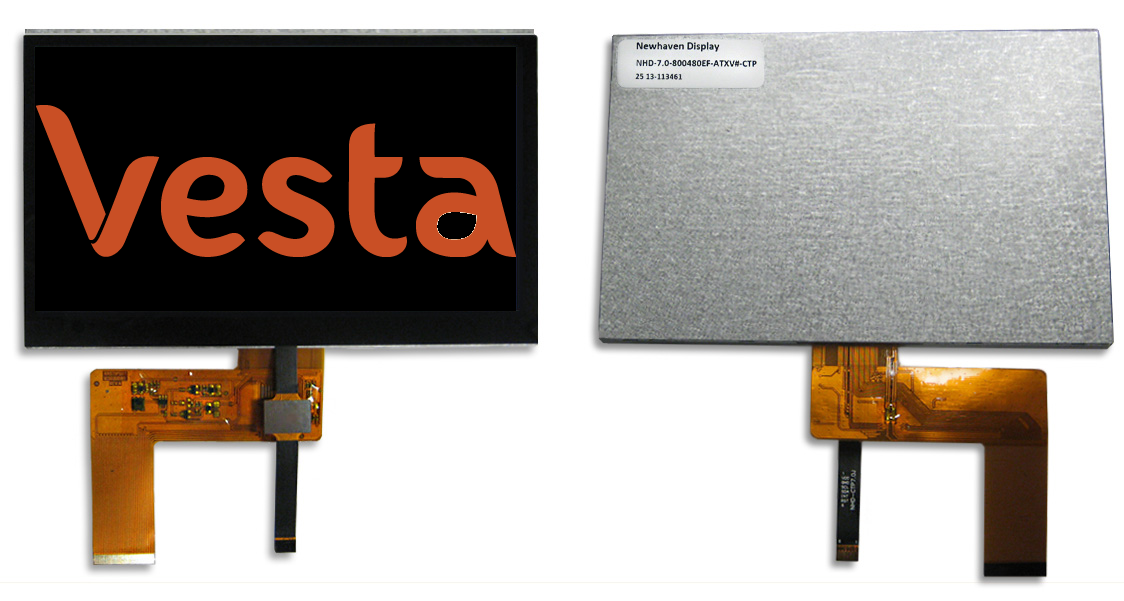
\includegraphics[width=0.5\textwidth,keepaspectratio]{chap/hardFig/newhaven_screen_image}
     \caption{Screen package.}
     \label{fig:screen package}
 \end{figure}

 Individual components are discribed in the following sub chapters.

\subsubsection{Screen}
The screen is the NHD-7.0-800480EF-ATXV\#-CTP from Newhaven Display. The specifications of the screens are listed bellow.
\begin{itemize}
  \item {7" Diagonal}
  \item{Resolution: 800xRGBx480}
  \item{24 bit digital RGB interface}
  \item{White led backlight}
  \item{55-65$^{\circ}$ Top-bottom viewing angle }
  \item{70 $^{\circ}$ left-rigth viewing angle}
\end{itemize}


\subsubsection{Touchscreen}

\begin{itemize}
  \item {Capacitive touch panel with built-in Focaltech ft5x06 controller}
  \item {i2c interface}
  \item {linux kernel compatible}
\end{itemize}
The touchpanel is very smooth and reactive. The
\subsubsection{Backlight}
The backlight is a quite bright white led array consisting of 5x3 LEDs. the configuration can be seen in fig.\ref{fig:backlight_led}

\begin{figure}[!htb]
    \centering
    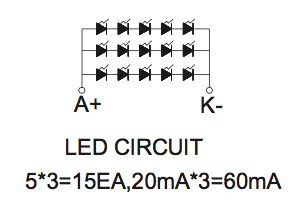
\includegraphics[width=0.5\textwidth,keepaspectratio]{chap/hardFig/backlight_led_circuit}
    \caption{Backlight LED array configuration.}
    \label{fig:backlight_led}
\end{figure}

This LED array requires 60 mA at 16 V to operate. This power is taken directly from the 3.3v of the BBB and boosted to the required voltage by FAN5333A LED driver from Fairchild semiconductors.
This IC is a general purpose LED driver which can be controller with a PWM imput.
Our implementation of the FAN5333A is pictured in fig.\ref{fig:backlight driver schematics}.

\begin{figure}[!htb]
    \centering
    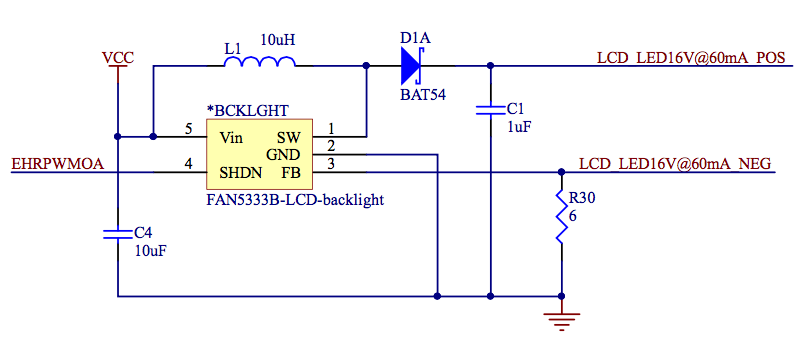
\includegraphics[width=0.7\textwidth,keepaspectratio]{chap/hardFig/backlight_led_driver_sch}
    \caption{FAN5333A Backlight LED driver implementation.}
    \label{fig:backlight driver schematics}
\end{figure}

From the data sheet the resistance R30 sets the current. The net EHRPWMMOA is connected to a pwm pin on the BBB.
\subsection{Wireless Communication}
Our device has to connect to the internet over a WLAN to download new messages from the website. We chose to use the WL1835 chip from Texas instruments. This IC integrates WlAN, 4.1 bluetooth and BLE. An important point is that TI provides support for the linux kernel we are using and the AM335x 1GHz ARM® Cortex-A8.

\begin{figure}[!htb]
    \centering
    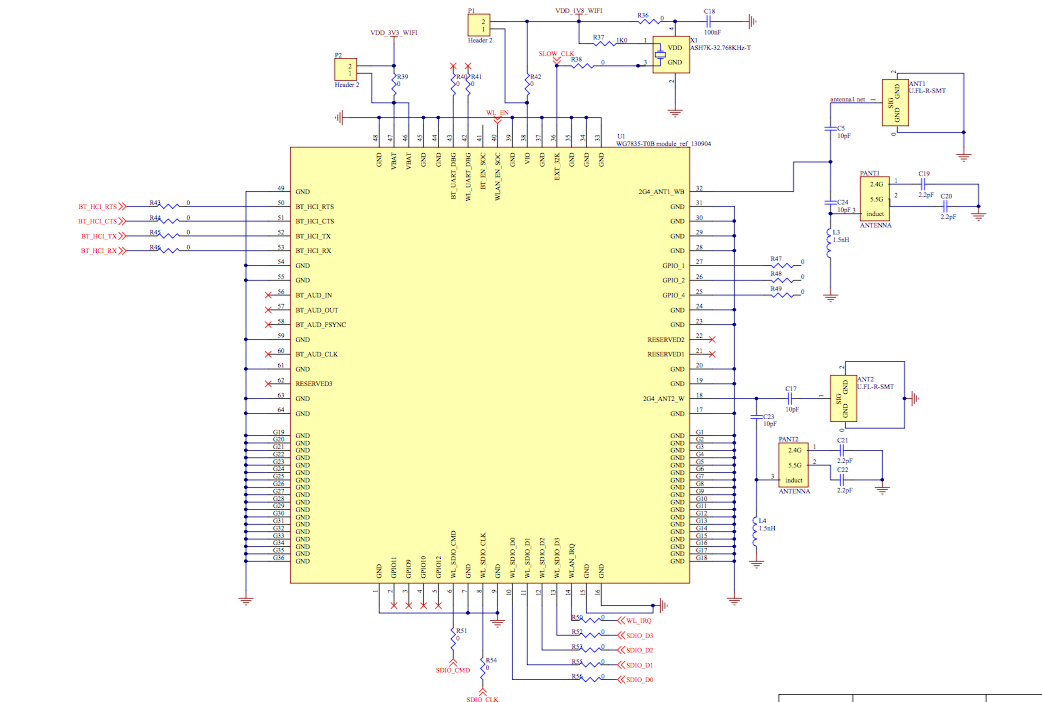
\includegraphics[width=1\textwidth,keepaspectratio]{chap/hardFig/wl1835_chip_sch}
    \caption{Wl1835 implementation.}
    \label{fig:wl1835 chip}
\end{figure}

\subsubsection{Wlan}
The chip supports the IEEE standards 802.11a/b/g/n. This means it can provide up to 100 MPs with UDP and up to 80 MPs with TCP.
It uses a 4 bit SDIO interface to communicate with the BBB. The BBB has 2 SDIO interfaces which are used to communicate with the $\mu$
 Sd card and the onboard EMMC. Therefore using the wl1835 means that we no longer have acces to the emmc. This is not a big issue as the operating system can be located on the sd card.

\subsubsection{Bluetooth}
The Wl1835 provides 4.1 bluetooth and low energy bluetooth capabilities. Uart host controlled interface is used here.
\subsubsection{Power management}
The WL1835 is quite power hungry and requires both 3.3V and 1.8V to operate. Therefore it has its own linear regulators.
\subsection{Front LED}
The LED is there to inform the user of a new message. Therefor it could be quite low power. Seeedstudio only had an RGB LED which we ordered although for the final led we will use is a warm white single color LED.

We want it to flash in a heartbeat patern. This is achieved by using a PWM pin of the BBB
\subsection{Power management}
\subsection{Batteries and charger}
\subsection{PCB}
\subsection{Cost estimates}
